\documentclass[tikz,border=5pt]{standalone}
\usepackage[T1]{fontenc}
\usetikzlibrary{arrows.meta,positioning,fit,backgrounds}

\definecolor{lzero}{HTML}{365A7C}
\definecolor{lone}{HTML}{497F9C}
\definecolor{ltwo}{HTML}{5CA5BE}
\definecolor{lthree}{HTML}{84C7D8}
\definecolor{ink}{HTML}{243746}

\begin{document}
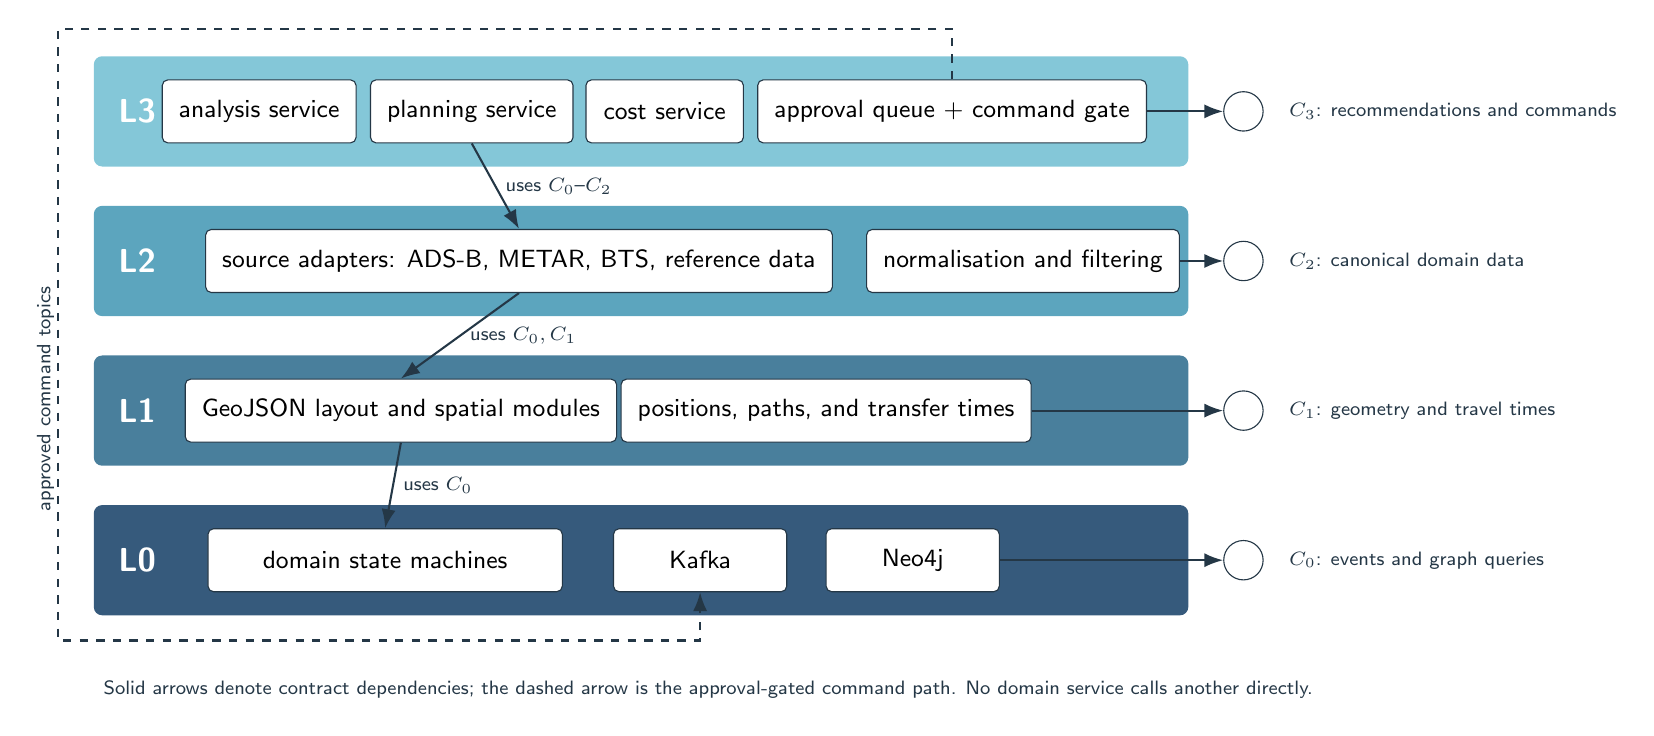
\begin{tikzpicture}[
  font=\sffamily\small,
  component/.style={draw=ink, rounded corners=2pt, fill=white,
                    minimum height=8mm, align=center, inner xsep=6pt},
  contract/.style={draw=ink, circle, fill=white, minimum size=5mm, inner sep=0pt},
  dependency/.style={-{Latex[length=2.4mm]}, line width=.75pt, ink},
  command/.style={-{Latex[length=2.4mm]}, dashed, line width=.75pt, ink},
  layerlabel/.style={font=\sffamily\bfseries\large, text=white},
  note/.style={font=\sffamily\scriptsize, text=ink, align=left}
]

% Layer backgrounds
\fill[lthree,rounded corners=3pt] (0,6.3) rectangle (13.9,7.7);
\fill[ltwo,rounded corners=3pt]   (0,4.4) rectangle (13.9,5.8);
\fill[lone,rounded corners=3pt]   (0,2.5) rectangle (13.9,3.9);
\fill[lzero,rounded corners=3pt]  (0,0.6) rectangle (13.9,2.0);

\node[layerlabel] at (.55,7.0) {L3};
\node[layerlabel] at (.55,5.1) {L2};
\node[layerlabel] at (.55,3.2) {L1};
\node[layerlabel] at (.55,1.3) {L0};

% Components
\node[component,minimum width=2.2cm] (analysis) at (2.1,7.0) {analysis\ service};
\node[component,minimum width=2.2cm] (planning) at (4.8,7.0) {planning\ service};
\node[component,minimum width=2.0cm] (cost) at (7.25,7.0) {cost\ service};
\node[component,minimum width=3.3cm] (approval) at (10.9,7.0) {approval queue\ + command gate};

\node[component,minimum width=7.8cm] (adapters) at (5.4,5.1)
  {source adapters: ADS-B, METAR, BTS, reference data};
\node[component,minimum width=2.8cm] (normalise) at (11.8,5.1)
  {normalisation\ and filtering};

\node[component,minimum width=4.8cm] (geometry) at (3.9,3.2)
  {GeoJSON layout and spatial modules};
\node[component,minimum width=4.8cm] (travel) at (9.3,3.2)
  {positions, paths, and transfer times};

\node[component,minimum width=4.5cm] (domains) at (3.7,1.3)
  {domain state machines};
\node[component,minimum width=2.2cm] (kafka) at (7.7,1.3) {Kafka};
\node[component,minimum width=2.2cm] (neo4j) at (10.4,1.3) {Neo4j};

% Provided-interface symbols and labels
\node[contract] (c0) at (14.6,1.3) {};
\node[note,right=2mm of c0] {\textbf{$C_0$}: events and graph queries};
\node[contract] (c1) at (14.6,3.2) {};
\node[note,right=2mm of c1] {\textbf{$C_1$}: geometry and travel times};
\node[contract] (c2) at (14.6,5.1) {};
\node[note,right=2mm of c2] {\textbf{$C_2$}: canonical domain data};
\node[contract] (c3) at (14.6,7.0) {};
\node[note,right=2mm of c3] {\textbf{$C_3$}: recommendations and commands};

\draw[dependency] (neo4j.east) -- (c0.west);
\draw[dependency] (travel.east) -- (c1.west);
\draw[dependency] (normalise.east) -- (c2.west);
\draw[dependency] (approval.east) -- (c3.west);

% Contract consumption between layers
\draw[dependency] (geometry.south) -- node[note,right]{uses $C_0$} (domains.north);
\draw[dependency] (adapters.south) -- node[note,right]{uses $C_0,C_1$} (geometry.north);
\draw[dependency] (planning.south) -- node[note,right]{uses $C_0$--$C_2$} (adapters.north);

% Only the gated command interface closes the loop. Route it around the
% component stack so the return path does not obscure any layer contents.
\draw[command] (approval.north) -- (10.9,8.05) -- (-.45,8.05)
  -- (-.45,.28) -- (7.7,.28) -- (kafka.south);
\node[note,rotate=90,anchor=south] at (-.38,3.35)
  {approved command topics};

\node[note,anchor=west] at (0,-.35)
  {Solid arrows denote contract dependencies; the dashed arrow is the approval-gated command path. No domain service calls another directly.};

\end{tikzpicture}
\end{document}
